\documentclass[a4paper,fontsize = 8pt]{scrartcl}
\usepackage[nswissgerman]{babel}

% 3 column landscape layout with fewer margins
\usepackage[landscape, left=0.75cm, top=1cm, right=0.75cm, bottom=1.5cm, footskip=15pt]{geometry}
\usepackage{flowfram}
\ffvadjustfalse
\setlength{\columnsep}{1cm}
\Ncolumn{3}

% define nice looking boxes
\usepackage[many]{tcolorbox}

% a base set, that is then customised
\tcbset {
  base/.style={
    boxrule=0mm,
    leftrule=1mm,
    left=1.75mm,
    arc=0mm, 
    fonttitle=\bfseries, 
    colbacktitle=black!10!white, 
    coltitle=black, 
    toptitle=0.75mm, 
    bottomtitle=0.25mm,
    title={#1}
  }
}

\definecolor{nicegreen}{rgb}{0.004, 0.5, 0.35}
\newtcolorbox{mainbox}[1]{
  colframe=nicegreen, 
  base={#1}
}

\newtcolorbox{subbox}[1]{
  colframe=black!20!white,
  base={#1}
}

% Mathematical typesetting & symbols
\usepackage{amsthm, mathtools, amssymb} 
\usepackage{marvosym, wasysym}
\usepackage{derivative}
\allowdisplaybreaks

% Tables
\usepackage{tabularx, multirow}
\usepackage{booktabs}

% Make enumerations more compact
\usepackage{enumitem}
\setitemize{itemsep=0.5pt}
\setenumerate{itemsep=0.75pt}
\setlength{\parindent}{0pt}

% To include sketches & PDFs
\usepackage{graphicx}

% For hyperlinks
\usepackage{hyperref}
\hypersetup{
  colorlinks=true
}

% Metadata
\title{Cheatsheet Analysis 2}
\author{Nicolas Wehrli}
\date{January 2023}

% Math helper stuff
\def\limn{\lim_{n\to \infty}}
\def\limxo{\lim_{x\to 0}}
\def\limxi{\lim_{x\to\infty}}
\def\limxn{\lim_{x\to-\infty}}
\def\sumk{\sum_{k=1}^\infty}
\def\sumn{\sum_{n=0}^\infty}
\def\R{\mathbb{R}}
\def\C{\mathbb{C}}
\def\Q{\mathbb{Q}}
\def\N{\mathbb{N}}
\def\X{\mathcal{X}}
\def\dx{\text{ d}x}

\begin{document}

\maketitle

\section{Differential equations}
\begin{mainbox}{Ordinary Differential Equation (ODE)}
    In general an \textbf{ordinary} differential equation (ODE) relates a function $f(x)$ at $x$ to the values of its derivatives at $x$.
    I.e. it's an equation of the Form $$F(x, f(x), f'(x), f''(x), ..., f^{(n)}(x)) = 0$$ 
    The order of the diff. equation is the highest order of derivative that appears in the equation.

    A partial diff. equation is a diff. equation for a function of several variables. (It involves "partial derivatives").
\end{mainbox}
$f'(x+2) = f(x)$ is not an \textbf{ordinary} differential equation.

\begin{mainbox}{Linear ODE}
    A linear ODE of order $k$ on $I$, is an equation of the form $$y^{(k)} + a_{k-1}(x)y^{(k-1)}+...+a_1(x)y'+a_0(x)y = b(x)$$ 
    where $b, a_1, ..., a_{k-1}$ are continous functions of $x$ defined on $I$ with values in $\C$.

    If $b(x) = 0, \forall x \in I$, we call the ODE \textbf{homogeneous} and otherwise \textbf{inhomogeneous}. 
\end{mainbox}

\subsection*{Recognising a linear ODE}
\begin{itemize}
    \item no coefficients before the highest order derivative (\textbf{what about constants?})
    \item alle coefficients are continous functions
    \item no products of $y$ and it's derivatives
    \item $y$ and all of it's derivatives occur with the power one
    \item Neither $y$ nor it's derivatives are \textit{inside} another function.
\end{itemize}

\begin{mainbox}{Solutions of Linear ODE's}
    Let $I \subset \R$ open interval, $k \geq 1, k \in \N$.
    $$y^{(k)}+a_{k-1}y^{(k-1)} + ... + a_0y = b$$
    is a linear ODE over $I$ with continous coefficients.
    
    Then
    \begin{enumerate}
        \item The set of solutions $S_0$ for the associated \textbf{homogeneous} ODE (when $b = 0$), is a vector space of dimension $k$.
        \item For any initial conditions (i.e. any choice of $x_0 \in I$ and $(y_0, ..., y_{k-1}) \in \C^k$) there exists an \textbf{unique} solution $f \in S_0$ s.t. $f(x_0) = y_0, f'(x_0) = y_1, ..., f^{(k-1)}(x_0) = y_{k-1}$.
        \item For any arbitrary $b(x)$, the set of solutions of the ODE is $$S_b = \{f + f_p \mid f \in S_0\}$$ where $f_p$ is a \textbf{paritcular} solution of the ODE.
        \item For any initial condition there is a unique condition there is a unique solution $f \in S_b$.
    \end{enumerate}
     $S_b$ is \textbf{not} a Vector Space! (It's an affine Space.)
\end{mainbox}

\subsection{Linear ODE's of order 1}
$I \subset \R$ be an open interval.

We consider the diff. equation of the form \[y' + a(x)y = b(x)\]
\begin{enumerate}
  \item (Homogeneous solution) 
  \begin{align*}
    y' + a(x)y &= 0\\
    \frac{y'}{y} &= -a(x) \quad (\text{assuming } y \neq 0, \forall x \in I)\\
    \ln(|y|) &= -A(x)+C\\
    y &= e^C \cdot e^{-A(x)} = Ke^{-A(x)}, K \in \C
  \end{align*}
  If an initial condition is given, we can determine $K$.
  \item (Particular solution) 
  
  Use either ``Variation of parameters'' or ``Educated guess''.
\end{enumerate}
\subsection{Variation of parameters}
We assume that the particular solution is of the form \(f_p = K(x)e^{-A(x)}\) for a function \(K: I \to \C\). Then we can insert our guess into the ODE and see what it forces $K$ to satisfy. We get 
    \begin{align*}
        b(x) &= (K(x)e^{-A(x)})' + a(x)(K(x)e^{-A(x)})  \\
        b (x) &= K'(x)e^{-A(x)} - a(x)K(x)e^{-A(x)} + a(x)K(x)e^{-A(x)} \\
        b(x)  &= K'(x)e^{-A(x)} \\
        K'(x) &= b(x)e^{A(x)}
    \end{align*}
    and thus \[K(x) = \int_{x_0}^x b(t) e^{A(t)} \mathop{dt}\] Therefore we get \[f_p = \left(\int_{x_0}^x b(t) e^{A(t)} \mathop{dt}\right) \cdot e^{-A(t)}\]
    The method with the ``Integration factor'' gives the same particular solution!
\subsection{Educated Guess for general case}
\begin{enumerate}[label = (\arabic*)]
    \item If $b(x) = x^de^{\beta x}$ and $\beta$ \textbf{is not a root of the companion Polynomial $P$}, then we try $f_p(x) = Q(x)e^{\beta x}$, where $Q$ is a Polynomial of degree $d$.
    \item If $b(x) = x^d\cos(\beta x)$ or $b(x) = x^d\sin(\beta x)$ and $\beta$ \textbf{is not a root of the companion Polynomial $P$}, we try \[f_p(x) = Q_1(x)\cos(\beta x) + Q_2(x)\sin(\beta x)\] where $Q_1, Q_2$ are polynomials of degree $d$.
    \item If $b$ is of the form of the previous two examples but $\beta$ \textbf{is a root with multiplicity $j$ of the companion polynomial}, then one tries the same functions, except that the Polynomials $Q$ (or $Q_1, Q_2$ resp.) have degree $d+j$.
    \item The special case $\beta = 0$ in cases $(1), (2), (3)$ corresponds to the situation where $b$ is a polynomial of degree $d$. Therefore we try $f_p$ as a polynomial of degree $d$, unless $0$ is a root with multiplicity $j$, then we try $f_p$ as a polynomial of degree $d+j$.
\end{enumerate}


\subsection{Educated Guess for constant coefficients}

If $b(x)$ is of a specific form, we try following $f_p$, where we insert the $f_p$ into the ODE, which gives us a system of equations for the constants:

\begin{center}
  \renewcommand*{\arraystretch}{1.6}
  \begin{tabular}{cc} 
    \toprule
    $b(x)$ & Ansatz \\ 
    \midrule
    $a \cdot e^{\alpha x}$ & $b \cdot e^{\alpha x}$\\
    $a \sin(\beta x)$ & $c \sin(\beta x) + d \cos(\beta x)$\\
    $b \cos(\beta x)$ & $c \sin(\beta x) + d \cos(\beta x)$\\
    $a e^{\alpha x} \sin(\beta x)$ & $e^{\alpha x} \Big( c \sin(\beta x) + d \cos(\beta x) \Big)$\\
    $b e^{\alpha x} \cos(\beta x)$ & $e^{\alpha x} \Big( c \sin(\beta x) + d \cos(\beta x) \Big)$\\
    $P_n(x) \cdot e^{\alpha x}$ & $R_n(x) \cdot e^{\alpha x}$\\
    $P_n(x) \cdot e^{\alpha x} \sin(\beta x)$ & $e^{\alpha x} \left( R_n(x) \sin(\beta x) + S_n(x) \cos(\beta x) \right)$\\
    $P_n(x) \cdot e^{\alpha x} \cos(\beta x)$ & $e^{\alpha x} \left( R_n(x) \sin(\beta x) + S_n(x) \cos(\beta x) \right)$\\
    \bottomrule
  \end{tabular}
\end{center}

\(P_n, R_n \) and \(S_n\) are Polynomials of degree $n$. 

\begin{enumerate}
  \item If \(b(x)\) is a linear combination of any of the base functions, try that linear combination of 'Ansatz' functions.  
  \item If $b(x) = c \cdot e^{\alpha x}, \alpha \in \C$ for which $\alpha$ is a zero of the characteristic polynomial (i.e. $\alpha$ is a root and $b(x)$ a solution for the homogeneous equation), then we try $f_p = d \cdot x^m \cdot e^{\alpha x}$, where $m$ is the multiplicity of the root $\alpha$.
\end{enumerate}

\subsection{Linear ODE's with constant coefficients}
We consider an ODE of the form
\[y^{(k)} + a_{k-1} y^{(k-1)} + \ldots + a_1 y' + a_0 y = b(x)\]
We search for a homogeneous solution of the form \(e^{\lambda x}\). Now we can solve the characteristic polynomial:
\begin{align*}
  P(\lambda) = e^{\lambda x} \left(\lambda^k + a_{k-1}\lambda^{k-1} + \ldots + a_0\right) = 0 \\ 
  \implies 0 = \lambda^k + a_{k-1}\lambda^{k-1} + \ldots+ a_0
\end{align*}
\begin{itemize}
    \item The roots of \(P(\lambda)\) are the Eigenvalues \(\lambda_i\), with corresponding multiplicity \(m_r\). Thus the functions \(f_{i,r} : x \to x^r e^{\lambda_i x}, 0 \leq r < m_r\) span the Vector Space \(S_0\).
    \item If \(\lambda = \beta + \gamma i\) is a complex of \(P(\lambda)\), then the complex conjugation, i.e. \(\bar{\lambda} = \beta - \gamma i\) is also a root. Thus \(f_1 = e^{\lambda x}\) and \(f_2 = e^{\bar{\lambda} x}\) are solutions to the homogeneous equation.
    \item We realize that \(f_1 = e^{\lambda x} = e^{\beta x} (\cos(\gamma x)+ i \sin(\gamma x))\) and \(f_2 = e^{\bar{\lambda} x}= e^{\beta x} (\cos(\gamma x) - i \sin(\gamma x))\).
    \item We can thus replace $f_1$ and $f_2$ by \(\tilde{f_1} = e^{\beta x} \cos(\gamma x)\) and \(\tilde{f_2} = e^{\beta x} \sin(\gamma x)\). (Note that $f_1 = \tilde{f_1} + i \tilde{f_2}$ and $f_2 = \tilde{f_1} - i \tilde{f_2}$)
    \item Note that we are often only interested in finding real-valued solutions if the coefficients are all real valued.
    \item If \(y^{(k)} + a_{k-1}y^{(k-1)} + \dots + a_0 y = 0\) only has real coefficients, every pair of complex conjugated roots $\beta_j \pm \gamma_j i$ with multiplicity $m_j$ leads to a solution \[x^l e^{\beta_j x} \Big( \cos(\gamma_j x) + i \sin(\gamma_j x) \Big) \quad \text{for }0 \leq l < m_j\]
    of which then the real part can be extracted.
\end{itemize}
To find a particular solution $f_p$ we can as in the general case use \textbf{Varation of parameters} or \textbf{Educated guess}. We will now show an simple example with $2$ basis functions:

Consider the Linear ODE $y'' + y a_1y' + a_0y = b$
\begin{enumerate}[label=(\arabic*)]
  \item Assume the space of homogeneous solutions $S_0$ is spanned by $f_1, f_2$, i.e. $f_0 = f_1 + f_2$ is also a solution  
  \item Now we try \(f_p = z_1(x) f_1 + z_2(x) f_2\)
  \item We first insert $f_p$ into the ODE and we require the additional constraint that $ z_1'(x) f_1 + z_2'(x) f_2 = 0$ to find a concrete solution. 
  
  Therefore we get the following system of equations:
  \begin{align*}
    z_1'(x) f_1 + z_2'(x) f_2 &= 0\\
    z_1'(x) f_1' + z_2'(x) f_2' &= b(x)\\
  \end{align*}
  We can solve this as follows:
  \begin{align*}
    W &= f_1 f_2' - f_2 f_1' \neq 0\\
    \Rightarrow z_1' &= \frac{-f_2 b}{W} \; , z_2' = \frac{f_1 b}{W}\\
    \Rightarrow f_p &= \left(\int \frac{-f_2 b}{W} dt\right)f_1  + \left(\int \frac{f_1 b}{W} dt\right)f_2 
  \end{align*}
\end{enumerate}

\subsection{Seperation of Variables}
    Consider a differential equation of the form 
    \begin{align*}
        y'(x) &= b(x)g(y)
    \end{align*}
    Assume $g(y(x)) \neq 0$. If $\exists y_0$ s.t. $g(y_0(x)) = 0$ then $y = y_0$ is a solution.
    \begin{align*}
        \frac{y'(x)}{g(y(x))} &= b(x)\\
        \int \frac{y'(x)}{g(y(x))} \mathop{dx} &= \int b(x) \mathop{dx}\\
    \end{align*}
    Applying substitution with $u = y(x)$ we obtain 
    $$\int \frac{1}{g(u)}\mathop{du} = \int b(x) \mathop{dx}$$
    We can then determine both integrals and solve for $u = y$.

\section{Derivations in \texorpdfstring{\(\R^n\)}{Rⁿ}}
\begin{subbox}{Monomial in $\R^n$}
  A Monomial of degree \(e\) is a function $f: \R^n \mapsto \R:$
  \begin{align*}
    (x_1, \ldots, x_n) \mapsto \alpha x_1^{d_1}\cdot \ldots \cdot x_n^{d_n} \\
    e = d_1 + \ldots + d_n 
  \end{align*}
  \(\to\) i.e. a Polynomial that only has one term.
\end{subbox}
\begin{mainbox}{Polynomial in $\R^n$}
  A Polynomial with \(n\) variables of degree \(d\) is a finite sum of Monomials of degree \(e \le d\).
\end{mainbox}

\subsection{Convergence}
\begin{enumerate}
  \item Dot product: \(\left< x,y\right> = \sum_{i=0} x_i \cdot y_i\)
  \item Euclidean norm: \(||x|| := \sqrt{x_2^1 + \cdots + x_n^2}\) with the following properties:
  \begin{enumerate}
    \item \(||x|| \ge 0, ||x|| = 0 \iff x = 0\)
    \item \(||\lambda x|| = |\lambda| \cdot ||x||, \forall \lambda \in \R\)
    \item \(||x+y|| \le ||x|| + ||y||\)
    \item \(|\left<x,y\right>| \le ||x|| \cdot ||y||\)
  \end{enumerate}
\end{enumerate}

\begin{mainbox}{Definition Convergence}
  Let \((x_k)_{k \in \mathbb{N}}, x_k \in \R^n\). The following definitions for \(\lim_{k\to\infty}x_k = y\) equivalent:
  \begin{enumerate}
    \item \(\forall \epsilon > 0 \exists N \ge 1\) such that \(\forall k \ge N \ ||x_k - y|| < \epsilon\).
    \item For every \(i, 1 \le i \le n\) the sequence \((x_{k,i})_k\) of real numbers converges to \(y_i\).
    \item The sequence \(||x_k - y||\) of real numbers converges to \(0\).
  \end{enumerate}
\end{mainbox}
\subsection{Continuity}
\begin{mainbox}{Definition Continuity}
    Let \(f: \X \subset \R^n \to \R^m\)  and \(x_0 \in \X\). 
    
    \(f\) is continous in \(x_0\), if one of the following conditions is fulfilled:
    \begin{enumerate}
        \item \(\forall \epsilon > 0 \ \exists \delta > 0\) such that for all \(x \in \X\) \[||x - x_0|| < \delta \implies ||f(x) - f(x_0)|| < \epsilon\]
        \item \(\forall\) sequences \((x_k)\) in \(X\) with \(\lim_{k \to \infty} x_k = x_0\) we have \[\lim_{k \to \infty} f(x_k) = f\left(\lim_{k \to \infty} x_k\right) = f(x_0)\]
    \end{enumerate}
\end{mainbox}
\(f\) is continous on \(\X\) $\iff$ \(f\) is continous at every point \(x_0 \in \X\). 

In Addition we have the following:
\begin{enumerate}
  \item Cartesian product of continous functions is continous.
  \item \(f: \R^n \mapsto \R^m\)\\
  \((x_1, \ldots, x_n) \mapsto (f_1(x),\ldots,f_m(x))\) \\is continous $\iff$ \(f_i: \R^n \to \R\) continous \(\forall i = 1, \ldots, m\).
  \item Linear Maps \(x \mapsto Ax\) are continous.
  \item Finite sums and products of continous functions are continous.
  \item Functions with seperated Variables are continous if each factor is continous. (i.e. $f(x_1,...,x_n) = f_1(x_1)f_2(x_2)\cdot...\cdot f_n(x_n)$ is continous if $f_1, f_2, ..., f_n$ are continous.)
  \item In particular Polynomials are continous.
  \item The composition of continous functions is continous.
  \item If $f: \R^2 \mapsto \R$ is continous. For an arbitrary fixed $y_0 \in \R$ we can define $g_{y_0}(x) := f(x, y_0)$. Since $g_{y_0}$ is a composition of continous functions it is also continous. 
  \item Warning! The converse is not true. $g_{y_0}$ continous for all $y_0 \in \R$ does \textbf{not} imply that  $f$ is continous!
\end{enumerate}
\begin{mainbox}{Sandwich-Lemma}
  If \(f, g, h: \R^n \to \R\) are functions with \(f(x) < g(x) < h(x) \\ \forall x \in \R^n\). Let $a \in \R^n$:
  \[\lim_{x\to a} f(x) = \lim_{x \to a} h(x) = L \implies \lim_{x\to a} g(x) = L\]
\end{mainbox}
\subsection{Properties of sets}
A set \(\X \subset \R^n \) is
\begin{itemize}
  \item \textbf{bounded}, if the set \(\{ ||x|| \mid x \in \X \}\) is bounded in \(\R\)(i.e. \(\exists K \ge 0, \forall x \in \X: ||x|| \le K\)).
  \item \textbf{closed}, if every sequence \((x_k)_{k\in \N} \subset \X\), that converges to some Vector \(y \in \R^n\), we have \(y \in \X\) (i.e. limits of sequences in $X$ are also in $X$).
  \item \textbf{compact}, if its closed and bounded.
  \item \textbf{open} if, for any $x =(x_1,x_2,...,x_n) \in \X$, there exists $\delta >0$ such that the set \[\{y = (y_1,...,y_n) \in \R^n \mid |x_i-y_i|< \delta, \forall 1 \leq i \leq n\}\] is contained in $\X$.
  \item \textbf{convex}, if \(\forall x, y \in \X: \lambda x + (1 - \lambda)y \in \X, \forall 0 \leq \lambda \leq 1\) (the line segment between \(x, y\) is contained in \(\X\)).
  \item \textbf{open}, if and only if the complement $Y = \R^n \setminus \X$ is \textbf{closed}. (Equivalent definition)
\end{itemize}
\textbf{Important examples:}
\begin{itemize}
  \item \((a,b) \subset \R\) is open.
  \item \(\left[a,b\right) \subset \R\) is neither open nor closed.
  \item \(\R^n\) and \(\varnothing\) are both open and closed. There exists no other set in $\R^n$ which is both open and closed.
  \item If $X \subseteq \R^n, Y \subseteq \R^m$ are both bounded (rsp. closed/compact) then $X \times Y \subseteq \R^{n+m}$ is bounded (rsp. closed/compact)
  \item In particular the cartesian product of compact intervals $I_i \in \R$: $I_1 \times I_2 \times ... \times I_n = \{(x_1,x_2,...,x_n) \in \R^n \mid x_i \in I_i\}$ is compact (i.e. closed and bounded).
  \item Let $f: \R^n \mapsto \R^m$ be continous. Then for every closed(/open) set $Y \subseteq \R^m$, the set $f^{-1}(Y)$ is closed(/open). 
\end{itemize}
\begin{subbox}{Bolzano-Weierstrass}
  Every bounded sequence in \(\R^n\) has a converging partial sequence.
\end{subbox}
\begin{subbox}{Min-Max-Theorem}
  Let \(\X \subset \R^n, \X \ne \varnothing\) be compact and \(f: \X \to \R\) a continous function. Then \(f\) is bounded and achieves a max and a min. I.e. $\exists x^+,x^- \in \X$, such that
  \[f(x^+) = \sup_{x\in \X} f(x) \quad f(x^-) = \inf_{x \in \X} f(x)\]
\end{subbox}

\subsection{Partial Derivatives}
\begin{mainbox}{Partial Derivative}
    To find the partial derivative of \(f: \X \subset \R^n \to \R\) (whereby \(\X\) open) with respect to $x_j, 1 \leq j \leq n$ at a point $x_0 \in \X$ we define:
\[\partial_j f (x_0)= \pdv{f}{x_{j}}(x_0) = \lim_{h \to 0} \frac{f(x_0 + h\cdot e_j) - f(x_0)}{h}\]where $e_j$ is the $j$-th canonical basis vector of $\R^n$.
\end{mainbox}
 
For \(f: \R^n \to \R^m, x_0 \in \R^n\) we have
\begin{align*}
  \pdv{f(x_0)}{x_j} := \begin{pmatrix}
    \pdv*{f_1(x_0)}{x_j}\\
    \vdots\\
    \pdv*{f_m(x_0)}{x_j}\\
  \end{pmatrix}
\end{align*}
Partial derivatives have following properties:
\begin{enumerate}
  \item \(\partial_j(f + g) = \partial_j (f) + \partial_j g\)
  \item \(\partial_j(f \cdot g) = \partial_j (f) \cdot g + \partial_j (g) \cdot f\)
  \item \(\partial_j(f / g) = \frac{\partial_j (f) \cdot g - \partial_j (g) \cdot f}{g^2}\) for \(g \ne 0\)
\end{enumerate}
\begin{mainbox}{Jacobi-Matrix}
Let \(f: \X \subset \R^n \to \R^m\) and \(\X\) an open set. The Jacobi-Matrix is the \(m \times n\) Matrix:
\[J_f = \left( \pdv{f_i}{x_j} \right)_{\substack{1 \leq j \leq n \\ 1 \leq i \leq m}}\]
\end{mainbox}
\begin{mainbox}{Gradient}
    In the special case of a function \(f: \X \subset \R^n \to \R\), the Jacobi-Matrix is a row vector which transposed gives us \(\nabla f\). The geometric interpretation is a vectorfield, defined by $\nabla f$, which indicates the direction and magnitude of the biggest growth of $f$. 
\end{mainbox}

% \begin{subbox}{Divergenz}
%   Die Divergenz einer Funktion \(f\) ist die Spur der Jacobi-Matrix von \(f\). \[\text{div}(f)(x_0) = \text{Tr}(J_f(x_0)) = \sum_{i=0}(J_f)_{i,i}\]
% \end{subbox}

\subsection{Differentiability}
\begin{mainbox}{Differentiability}
    Let $\X \subset \R^n$ be open, $x_0 \in \X$. We have 
    $f: \X \to \R^m$. 

    We say that $f$ is \textbf{differentiable} at $x_0$, with the differential $u$, if there exists a \textbf{linear map} $u: \R^n \to \R^m$ such that 
    \[\lim_{\substack{x \to x_0 \\ x \neq x_0}} \frac{f(x)-f(x_0)-u\cdot(x-x_0)}{||x-x_0||} = 0\]
    We denote $u = df(x_0) = d_{x_0}f$.
\end{mainbox}
\begin{itemize}
    \item If $f$ is differentiable at all points $x_0 \in \X$, then $f$ is differentiable on $\X$.
    \item Having all partial derivatives defined is not sufficient to conclude Differentiability.
    \item If all partial derivatives are defined and continous, then $f$ is differentiable.
\end{itemize}
\begin{mainbox}{Conclusions from Differentiability}
    If \(f,g\) are differentiable in \(x_0 \in \X\) we have:
    \begin{enumerate}
    \item \(f\) is continous in \(x_0\)
    \item \(f\) has all partial derivatives at \(x_0\) and the matrix of the linear map \(df(x_0): x \mapsto Ax\) is given by the \textbf{Jacobi-Matrix} of \(f\) at \(x_0\), i.e. \(A = J_f(x_0)\)
    \item \(d(f+g)(x_0) = df(x_0) + dg(x_0)\)
    \item If \(m = 1\), then \(f\cdot g\) is differentiable. If additionally \(g \ne 0\), then \(f/g\) is also differentiable. (Product rule and Quotient rule apply)
    \item (Chain rule): Let $\X \subseteq \R^n, Y \subseteq \R^m$ be open. 
    
    If \(f: \X \to Y, g: Y \to \R^p\) are both differentiable, we have \(d(g \circ f)(x_0) = dg(f(x_0)) \circ df(x_0)\). 
    Furthermore \[J_{g \circ f}(x_0) = J_g(f(x_0)) \cdot J_f(x_0)\]
    Therefore \[d(g \circ f)(x_0): \X \to \R^p \qquad x \mapsto J_g(f(x_0)) \cdot J_f(x_0) \cdot x\]
    \end{enumerate}
\end{mainbox}

\begin{subbox}{Tangent Space}
  The \textbf{tangent space} at $x_0$ of \(f\) is given by the graph of the affine linear map \(g(x) = f(x_0) + df(x_0)(x-x_0)\).
  
  I.e. \[\{(x,g(x)) \in \R^n\times\R^m \mid g(x) = f(x_0) + df(x_0)(x-x_0)\}\]
\end{subbox}

\begin{subbox}{Directional Derivative}
    Let $f: \X \subseteq \R^n \to \R^m$ be differentiable at $x_0 \in \X$.
    For any $v \in \R^n, v \neq 0$ the \textbf{directional Derivative} of $f$ at $x_0$ exists and is defined as 
    \[\partial_v f(x_0) = \lim_{h \to 0} \frac{f(x_0 + hv)-f(x_0)}{h} = J_f(x_0) \cdot v\] 
\end{subbox}
\begin{mainbox}{Change of variables (Bijection)}
    Let $\X \subset \R^n$ be open and $f: \X \to \R^n$ differentiable. $f$ is a \textbf{change of variable} around $x_0 \in \X$ if there exists a radius $r > 0$ such that the Ball 
    \[B_r(x_0) := \{x \in \R^n \mid ||x-x_0|| < r\}\] 
    has the property that the Image $Y = f(B_r(x_0))$ is open and there exists a differentiable map $g: Y \to B_r(x_0)$ such that $f \circ g = g \circ f =\text{id}$.

    We find that if det\((J_f(x_0)) \neq 0\) (i.e. $J_f(x_0)$ is invertible), then $f$ is a change of variables around $x_0$. Moreover the Jacobian of the inverse map $g$ is determined by \[J_g(f(x_0)) = J_f(x_0)^{-1}\]
    (Analog to the fact that a function $h: I \subseteq \R \to \R$ is bijective from $I$ to its image if $h' > 0$ or $h' < 0$)
\end{mainbox}
\subsection{Higher derivatives}
\subsubsection*{Notation for higher partial derivatives}
    
For a function $f: \R^n \to \R^t$ we denote higher order partial derivatives with the following:

    First let $m = (m_1, m_2, ..., m_n)$ and $|m| = m_1 + m_2 + ... + m_n$.

    We write
    \[\frac{\partial^{|m|}f_j}{\partial x_1^{m_1} \partial x_2^{m_2} \cdot ... \cdot \partial x_n^{m_n}} = \partial_{x^m}^{|m|}f_j, \ 1 \leq j \leq t\]


\begin{mainbox}{Differential Classes}
    Let \(\X \subset \R^n\) be open, $f : \X \to \R^m$. 
    \begin{itemize}
        \item We say that $f$ is differentiable of class $C^1$ if $f$ is differentiable on $\X$ and all its partial derivatives are continous. The set of all $C^1$ functions from $\X$ to $\R^m$ are denoted by $C^1(\X:\R^m)$.
        \item Let $k \geq 2$. We say $f \in C^k(\X:\R^m)$ (i.e. $f$ is of class $C^k$) if its differentiable and each $\partial_{x_i}f: \X \to \R^m$ ($1 \leq i \leq n$) is of class $C^{k-1}$.
        \item We say that $f$ is smooth or of class $C^\infty$ if $f \in C^k, \ \forall k \in \N$.
        \item All polynomials, trigonometric and exponential functions are of class $C^\infty$.
        \item If $f \in C^k, k \geq 2$ then all partial derivatives of order $\leq k$ are commutative.
        $$\pdv{f}{x_i, x_j} = \pdv{f}{ x_j, x_i}$$
    \end{itemize}
\end{mainbox}

\begin{mainbox}{Hessian}
    Let $\X \subset \R^n$ be open and $f: \X \to \R$ a $C^2$ function.

    For an $x_0 \in \X$, the \textbf{Hessian matrix} of $f$ at $x_0$ is the symmetric \(n \times n\) matrix that denotes the second derivative:
    \[\text{Hess}_f(x_0) := \left(\pdv{f(x_0)}{x_i, x_j}\right)_{1\le i,j \le n}\] 
    Sometimes we also denote it by $\nabla^2f(x_0)$ or $H_f(x_0)$.
\end{mainbox}
\subsection{Taylorpolynomials}
Sei \(k \le 1\) und \(f: \X \mapsto \R\) ist eine Funktion der Klasse \(C^k\) auf \(\X\). Sei \(x_0 \in \X\) fix. Das \(k\)-te Taylorpolynom von \(f\) am Punkt \(x_0\) ist das Polynom in \(n\) Variablen vom Grad \(\le k\):
\begin{align*}
  &T_k f(y; x_0) = f(x_0) + \sum_{i=1}^n \partial_i f(x_0) \cdot y_i + \dots \\
  &+ \sum_{m_1 + \cdots + m_n = k} \frac{1}{m_1! \cdots m_n!} \pdv{^k f(x_0) }{x_1^{m_1} \cdots \partial x_n^{m_n}} \cdot y_1^{m_1} \cdots y_n^{m_n}
\end{align*}

\subsubsection*{Beispiele}
\begin{align*}
  T_1 f(\vec{x}; x_0) &:= f(x_0) + \nabla f(x_0) \cdot \vec{x} \\
  T_2 f(\vec{x}; x_0) &:= T_1f + \frac{1}{2} \cdot \vec{x}^\top \cdot \text{Hess}_f(x_0) \cdot \vec{x}
\end{align*}

\subsection{Definit}
Eine symmetrische Matrix ist
\begin{itemize}
  \item \textbf{positiv definit}, falls alle Eigenwerte positiv sind.
  \item \textbf{negativ definit}, falls alle Eigenwerte negativ sind.
  \item \textbf{indefinit}, falls sowohl positive als negative Eigenwerte existieren.
\end{itemize}
Eigenwerte können mit dem charakteristischen Polynom gefunden werden:
\begin{align*}
  \text{det} \left(
  \begin{pmatrix}
    a & b\\
    c & d
  \end{pmatrix}
  -
  \begin{pmatrix}
    \lambda & 0\\
    0 & \lambda
  \end{pmatrix}
  \right)
  &=
  \text{det}
  \begin{pmatrix}
    a - \lambda & b\\
    c & d - \lambda
  \end{pmatrix}\\
  &\Rightarrow ad - (a + d) \lambda + \lambda^2 - bc = 0
\end{align*}
Für nichtsymmetrische Matrizen müssen wir für jeden Vektor \(v\) testen, ob \(v^\top A v > 0\) (bzw. \(< 0\)) gilt.
\subsubsection*{Determinante in drei Dimensionen}
\begin{align*}
  a \cdot \text{det}
  \begin{pmatrix}
    e & f\\
    h & i
  \end{pmatrix}
  - b \cdot \text{det}
  \begin{pmatrix}
    d & f\\
    g & i
  \end{pmatrix}
  + c \cdot \text{det}
  \begin{pmatrix}
    d & e\\
    g & h
  \end{pmatrix}
\end{align*}
\subsection{Extrema}
\subsubsection*{Lokale Extrema}
Sei \(f: \X \subset \R^n \mapsto \R\) differenzierbar und \(\X\) eine offene Menge. Dann ist \(x_0 \in \X\) ein lokales Maximum (Minimum) falls wir eine Umgebung \(B_r(x_0) = \{x\in \R^n \mid ||x-x_0|| < r \} \subset \X\) finden können, wo gilt:
\[\forall x \in B_r(x_0): f(x) \le (\ge) f(x_0)\]
Wenn \(x_0 \in \X\) ein lokales Extrema ist, dann gilt ausserdem \(\nabla f(x_0) = 0\).

\subsubsection*{Kritische Punkte}
Ein Punkt \(x_0 \in \X\) wo \(\nabla f(x_0) = 0\) gilt ist ein kritischer Punkt. Wenn \(\det(\text{Hess}_f(x_0)) \ne 0\), dann ist \(x_0\) nicht-degeneriert.

\subsubsection*{Sattelpunkt}
Wenn ein kritischer Punkt weder Maximum noch Minimum ist, dann nennen wir ihn Sattelpunkt.

\subsubsection*{Globale Extrema}
Sei \(f: K \mapsto \R\) und \(K\) kompakt, dann existiert ein globales Extrema von \(f\) und es ist entweder ein kritischer Punkt oder am Rand von \(K\). Um ein solches Extrema zu bestimmen, teilen wir \(K\) in sein Inneres \(\X\) und den Rand \(B\) auf. 

Nun bestimmen wir zuerst wie zuvor die kritischen Punkte von \(\X\). Um die Maximas/Minimas von \(B\) zu bestimmen, benötigen wir nur Wissen aus Analysis I (da von der Form \(\R \mapsto \R\)).
\subsubsection*{Testen von kritischen Punkten}
Sei \(f: \X \subseteq \R^n \mapsto \R, \X\) offen und \(f\in C^2\). Sei \(x_0\) ein nicht-degenerierter kritischer Punkt von \(f\). Dann gilt:
\begin{enumerate}
  \item $\text{Hess}_f(x_0)$ pos. def. \(\implies\) $x_0$ ist lokales Minimum.
  \item $\text{Hess}_f(x_0)$ neg. def. \(\implies\) $x_0$ ist lokales Maximum.
  \item $\text{Hess}_f(x_0)$ indefinit \(\implies\) $x_0$ ist Sattelpunkt.
\end{enumerate}
Dies funktioniert nicht, wenn \(x_0\) ein degenerierter kritischer Punkt ist. In einem solchen Fall müssen die Vorzeichen überprüft werden.
\subsubsection*{Kritische Punkte mit Nebenbedingungen}
Wenn wir Minimas/Maximas einer Funktion \(f: \X \mapsto \R\) mit einer Nebenbedingung \(g(x) = 0, g: \X \mapsto \R\) bestimmen wollen, können wir dafür Lagrange-Multiplikatoren verwenden.
\begin{subbox}{Lagrange-Multiplikator}
  Sei \(\X \subset \R^n\) offen und \(f,g: \X \mapsto \R\) Funktionen der Klasse \(C^1\). Wenn \(Y = \{x \in \X \mid g(x) = 0\) ist, dann ist \(x_0 \in Y\) ein lokales Extrema, welches die Nebenbedingung erfüllt, falls 
  \[\exists \delta > 0, f(y) \le (\ge) f(x_0), \quad \forall y \in B_\delta(x_0) \cap Y\]
  gilt. Nun ist entweder \(\nabla g(x_0) = 0\) oder \(\exists \lambda \in \R, \nabla f(x_0) = \lambda \cdot \nabla g(x_0)\), wobei \(\lambda\) dann Lagrange-Multiplikator gennant wird.
\end{subbox}
\section{Integrale in \texorpdfstring{\(\R^n\)}{Rⁿ}}
\subsection{Einfache Integrale}
Für \(f: \R \mapsto \R^n\) ist das Integral definiert als
\[\int_a^b f(t)dt = 
\begin{pmatrix*}
  \int_a^b f_1(t) dt \\
  \vdots\\
  \int_a^b f_n(t) dt
\end{pmatrix*}
\]

\begin{mainbox}{Kurve}
  Eine parametrisierte Kurve in \(\R^n\) ist eine stetige Ableitung \(\gamma: \left[a,b\right] \mapsto \R^n\) wobei \(\gamma\) stückweise in \(C^1\) ist, d.h. wir können \(\gamma\) so partitionieren, das alle Partitionen in \(C^1\) sind. Eine parametrisierte Kurve muss nicht injektiv sein.
\end{mainbox}
\subsection{Wegintegrale}
Sei \(\gamma : \left[a,b\right] \mapsto \R^n\) eine parametrisierte Kurve und \(\X \subset \R^n\) eine Menge, welche das Bild von \(\gamma\) beinhaltet. Sei \(f : \X \mapsto \R^n\) eine stetige Funktion. Dann ist ein Wegintegral (auch: Kurvenintegral) definiert als:
\[\int_\gamma f(s) ds = \int_a^b f(\gamma(t)) \cdot \gamma'(t) dt\]

Wegintegrale haben folgende Eigenschaften:
\begin{enumerate}
  \item Sie sind unabhängig von orientierungserhaltenden Reparametrisierungen, d.h. sie hängen nur vom Bild der Kurve und nicht von der Parametrisierung ab.
  \begin{align*}
    \gamma&: [a,\, b] \mapsto \R^n\\
    \tilde{\gamma}&: [c,\, d] \mapsto \R^n\\
    \varPhi&: [c, \, d] \mapsto [a, \, b]\\
    \tilde{\gamma} &= \gamma \circ \varPhi = \gamma(\varPhi)\\
    \Rightarrow &\int_\gamma f(s) \; ds = \int_{\tilde{\gamma}} f(s) \; ds
  \end{align*}
  \item Sei \(\gamma_1 + \gamma_2\) ein Pfad gegeben durch die Vereinigung zweier Kurven. Dann gilt
  \begin{align*}
    \gamma_1 + \gamma_2 &:=
    \begin{cases}
      \gamma_1(t) \quad& t \in [a, \, b]\\
      \gamma_2(t) \quad& t \in [b, \, d + b - c]
    \end{cases}\\
    \int_{\gamma_1 + \gamma_2} f(s) \; ds &= \int_{\gamma_1} f(s) \; ds + \int_{\gamma_2} f(s)\; ds
  \end{align*}
  \item Sei \(\gamma : \left[a,b\right] \mapsto \R^n\) ein Pfad und \(-\gamma\) ist der Pfad in die Gegenrichtung (d.h. \((-\gamma)(t) = \gamma(a + b - t)\)). Dann gilt
  \[\int_{-\gamma} f(s)ds = -\int_\gamma f(s) ds\]
\end{enumerate}

\subsection{Potential}
Ein differenzierbares skalares Feld \(g: \X \subset \R^n \mapsto \R\) mit \(\nabla g = f, f: \X \mapsto \R^n\) wird ein \textbf{Potential} von \(f\) genannt. Dies kann wie folgt verwendet werden:
\begin{align*}
  \int_\gamma f \; ds &= \int_a^b f(\gamma(t)) \cdot \gamma'(t) \; dt\\
  &= \int_a^b \nabla g(\gamma(t)) \cdot \gamma'(t) \; dt\\
  &= \int_a^b \frac{d}{dt} (g \circ \gamma) \; dt\\
  &= (g \circ \gamma)(b) - (g \circ \gamma)(a)
\end{align*}

\subsection{Konservative Vektorfelder}
Sei \(\X\) offen und \(f: \X \subset \R^n \mapsto \R^n\) ein stetiges Vektorfeld. Die folgenden Aussagen sind äquivalent:
\begin{enumerate}
  \item Falls für irgendwelche \(x_1, x_2 \in \X\) das Wegintegral \(\int_\gamma f(s) ds\) unabhängig von der Kurve in \(\X\) von \(x_1\) nach \(x_2\) ist, dann ist das Vektorfeld \(f\) konservativ.
  \item Jedes Wegintegral in \(f\) entlang einer geschlossenen Kurve (Schlaufe) ist 0.
  \item Ein Potential für \(f\) existiert.
\end{enumerate}
Es gilt ausserdem folgende notwendige, aber nicht ausreichende Bedingung:
\[f \text{ ist konservativ }\implies \pdv{f_i}{x_j} = \pdv{f_j}{x_i}\]

\begin{subbox}{Wegzusammenhängend}
  Sei \(\X \subset \R^n\) offen. \(\X\) ist wegzusammenhängend, falls für jedes Paar an Punkten \(x, y \in \X\) ein Pfad \(\gamma : \left(0,1\right] \mapsto \X\) existiert, der in \(C^1\) ist und \(\gamma(0) = x, \gamma(1) = y\) hält.
\end{subbox}

\begin{subbox}{Sternförmig}
  Eine Teilmenge \(\X \subset \R^n\) wird sternförmig genannt, falls \(\exists x_0 \in \X\) so dass \(\forall x \in \X\) eine Linie \(x_0\) nach \(x\) existiert, die komplett in \(\X\) enthalten ist. 
  \[\X \text{ ist konvex} \implies \X \text{ ist sternförmig}\]
\end{subbox}
Wenn \(\X\) eine sternförmige, offene Teilmenge von \(\R^n\) und \(f \in C^1\) ein Vektorfeld ist, dann gilt:
\begin{align*}
  \partial_j f_i = \partial_i f_j \quad \forall i,\, j
  \quad &\Rightarrow \quad \text{$f$ ist konservativ}\\
  \text{curl}(f) = \begin{pmatrix}
    0\\0\\0
  \end{pmatrix}
  \quad &\Rightarrow \quad \text{$f$ ist konservativ}
\end{align*}
\(\text{curl}(f)\) ist definiert als
\[\text{curl}(f) := \begin{pmatrix}
  \partial_y f_3 - \partial_z f_2 \\
  \partial_z f_1 - \partial_x f_3 \\
  \partial_x f_2 - \partial_y f_1
\end{pmatrix}\]
\subsection{Riemann-Integral in \texorpdfstring{\(\R^2\)}{R²}}
\begin{subbox}{Partition in zwei Dimensionen}
  Eine Partition \(P\) eines abgeschlossenen Rechtecks \(R = \left[a,b\right] \times \left[c,d\right]\) ist eine Menge von Rechtecken. Für jede Partition \(P_x : a = x_0 < \ldots < x_n = b\) von \(\left[a,b\right]\) und \(P_y\) (analog) erhalten wir eine Partition \(P_{i,j} = \left[x_{i-1}, x_i\right] \times \left[y_{j-1},y_j\right]\) von \(R\) mit der Fläche \(\mu({P_{i,j}} = (x_i - x_{i-1})(y_j - y_{j-1}))\).
\end{subbox}
Mit den Hilfsdefinitionen
\[f_{i,j} = \inf_{P_{i,j}} f(x,y), \quad F_{i,j} = \sup_{P_{i,j}} f(x,y)\]
können wir die Unter- und Obersumme bestimmen:
\begin{align*}
  s(P_x \times P_y) &= \sum_{i=1}^n \sum_{j=1}^m f_{i,j} \cdot \mu(P_{i,j}) \\
  S(P_x \times P_y) &= \sum_{i=1}^n \sum_{j=1}^m F_{i,j} \cdot \mu(P_{i,j})
\end{align*}
Sei \(f: R \mapsto \R\) beschränkt. \(f\) ist auf \(R\) integrierbar, falls \(\sup_{(P_x, P_y)} s(P_x, P_y) = \inf_{(P_x, P_y)} S(P_x, P_y)\) gilt. Dieser Wert ist dann definiert als:
\[\int_R f(x,y) \mathop{d(x,y)} \text{ oder } \int\int_R f(x,y) \mathop{d(x,y)}\]

\subsubsection*{Nicht-Quadratische Flächen}
Sei \(A \subset R\) eine Fläche. \(f : A \subset R \mapsto \R\) ist auf \(A\) integrierbar, falls \(f \cdot \X_A\) auf \(R\) integrierbar ist. 
\[\int_R f(x,y) \cdot \X_A(x,y) \mathop{d(x,y)} \text{ oder } \int_A f(x,y) \mathop{d(x,y)}\]
\(\X_A\) ist die charakteristische Funktion von \(A\).

\subsubsection*{Eigenschaften des Integrals}
Sei \(f,g : A \subset R \mapsto \R\) auf \(A\) integrierbar, dann gilt folgendes:
\begin{enumerate}
  \item \(\alpha, \beta \in \R: \alpha f + \beta g\) ist integrierbar:
  \[\int_A \alpha f + \beta g \mathop{d(x,y)} = \alpha \int_A f \mathop{d(x,y)} + \beta \int_A g \mathop{d(x,y)}\]
  \item Falls \(\forall (x,y) \in A: f(x,y) \le g(x,y)\), dann gilt:
  \[\int_A f(x,y) \mathop{d(x,y)} \le \int_A g(x,y) \mathop{d(x,y)}\]
  \item Falls \(f(x,y) \ge 0\) und \(B \subset A\), dann gilt:
  \[\int_B f(x,y) \mathop{d(x,y)} \le \int_A f(x,y) \mathop{d(x,y)}\]
  \item Dreiecksungleichung:
    \[\left| \int_A f(x,y) \mathop{d(x,y)}\right| \le \int_A \left|f(x,y)\right| \mathop{d(x,y)}\]
  \item Falls \(f = 1\), dann gilt:
  \[\int_A f(x,y) \mathop{d(x,y)} = \int_A 1 \mathop{d(x,y)} = \gamma(A)\]
\end{enumerate}


\begin{mainbox}{Satz von Fubini}
  Für eine Region \(D \subset \R^2 := \{\left(x,y\right) \mid a \le x \le b, g(x) < y < h(x)\}\) gilt:
  \[\int_D f(x,y)\mathop{dx} \mathop{xy} = \int_a^b \left(\int_{g(x)}^{h(x)} f(x,y) \mathop{dy}\right)\mathop{dx}\]
  Für eine Region \(D \subset \R^2 := \{ \left(x,y\right) \mid c \le y \le d, G(y) < x < H(y)\) gilt:
  \[\int_D f(x,y) \mathop{dx} \mathop{dy} = \int_c^d \left(\int_{G(y)}^{H(y)} f(x,y)\mathop{dx}\right) \mathop{dy}\]
\end{mainbox}
\begin{subbox}{Satz von Stolz}
  Sei \(f: R \mapsto \R\) integrierbar auf \(R = \left[a,b\right] \times \left[c,d\right]\). Sei \(y \mapsto f(x,y)\) integrierbar auf \(\left[c,d\right]\) für jedes \(x \in \left[a,b\right]\). Dann folgt:
  \[\int_R f(x,y) \mathop(d(x,y)) = \int_a^b \left(\int_c^d f(x,y) \mathop{dy}\right) \mathop{dx}\]
\end{subbox}
\begin{mainbox}{Nullmenge}
  Eine Nullmenge \(X \subset R \subset \R^2\) ist eine Menge, so dass für alle \(\epsilon > 0\) eine endliche Menge an Rechtecken \(R_k, 1 \le k \le n\) existiert, so dass:
  \[X \subset \bigcup_{k = 1}^n R_k, \; \sum_{k = 1}^n \mu (R_k) < \epsilon\]
  (Informell: Wir können die ganze Menge mit einer endlichen Menge an Rechtecken beliebiger Grösse überdecken.)
\end{mainbox}

\subsubsection*{Weitere Integrationskriterien}
\begin{enumerate}
  \item Sei \(R\) ein kompaktes Rechteck und \(f: R \mapsto \R\) ist stetig. Dann ist \(f\) integrierbar auf \(R\).
  \item Sei \(f: R \mapsto \R\) beschränkt und \(X\) die Menge aller nicht stetigen Punkte von \(f\). Wenn \(X\) eine Nullmenge ist, dann ist \(f\) auf \(R\) integrierbar.
  \item Sei \(\varphi_1, \varphi_2: \left[a,b\right]\mapsto \R\) stetig mit \(\forall x \in \left[a,b\right]: \varphi_1(x) \le \varphi_2(x)\) und \(A = \{(x,y)\mid a\le x \le b, \varphi_1(x) \le y \le \varphi_2(x)\}\). Falls \(f: A \mapsto \R\) stetig ist, so ist \(f\) auf \(A\) integrierbar und es folgt dass
  \[\int_A f(x,y) \mathop{d(x,y)} = \int_a^b \left(\int_{\varphi_1(x)}^{\varphi_2(x)} f(x,y) \mathop{dy}\right) \mathop{dx}\]
\end{enumerate}

\begin{subbox}{Lipschitz-Kurve}
  Eine Kurve \(\varphi : \left[0, 1\right] \mapsto \R^2\) ist Lipschitz, falls
  \[||\varphi(s) - \varphi(t)|| \le M \cdot |s-t| \ \forall s,t \in \left[0,1\right]\]
  Es folgt ausserdem, dass \(\varphi(\left[0,1\right]) \subset \R^2\) eine Nullmenge ist.
\end{subbox}

\subsection{Variablenwechsel}
Sei \(\partial A\) der Rand einer Menge \(A\):
\begin{align*}
    \partial A = \Big\{ &(x,y) \in \R^2 \mid \forall \delta > 0, \\ &R = (x - \delta, x + \delta) \times (y - \delta, y + \delta), \\
    &A \cap R \neq \emptyset \text{ und } \R^2 \backslash A \cap R \neq \emptyset \Big\}
\end{align*}

Sei \(\varphi : B \mapsto A\) eine stetige Abbildung, wobei \(A= A_0 \cup \partial A, \) \(B = B_0 \cup \partial B\) kompakte Mengen mit \(A_0, B_0\) offen und \(\partial A, \partial B\) Nullmengen sind. Wenn \(\varphi : B \setminus \N \mapsto A\) injektiv ist und \(N \subset B\) die Nullmenge ist, dann folgt
\[\int_A f(x,y) \mathop{d(x,y)} = \int_B f(\varphi(u,v)) \cdot \left|\det J_\varphi (u,v)\right| \mathop{d(u,v)}\]
\begin{enumerate}
  \item Polarkoordinaten: \(\mathop{dx}\mathop{dy} = r \mathop{dr} \mathop{d\theta}\)
  \item Zylindrische Koordinaten: \(\mathop{dx} \mathop{dy} \mathop{dz} = r \mathop{dr} \mathop{d\theta} \mathop{dz}\)
  \item Kugelkoordinaten: \(\mathop{dx}\mathop{dy}\mathop{dz} = r^2 \sin(\varphi) \mathop{dr} \mathop{d\theta} \mathop{d\varphi}\)
\end{enumerate}

\textbf{Achtung: Multiplikation mit der Determinante von Jacobi-Matrix nicht vergessen!}

\subsubsection*{Beispiel mit Kettenregel}
Sei \(f: \R^3 \mapsto \R\) eine glatte Funktion mit \(\nabla f \left(-\frac{\sqrt{3}}{2}, \frac{3}{2},7\right) = (6,2,0)\). Wenn wir nun \(\frac{\partial f}{\partial r}\left(\sqrt{3}, \frac{2}{3}\pi, 7\right)\) mit zylindrischen Koordinaten berechnen wollen, dann ist
\[\frac{\partial f(g(r,\theta,z))}{\partial r} = \frac{\partial f}{\partial x} \frac{\partial g_1}{\partial r} + \frac{\partial f}{\partial y} \frac{\partial g_2}{\partial r} + \frac{\partial f}{\partial z} \frac{\partial g_3}{\partial r}\]
Nun können wir die obige Information brauchen, um für \(\frac{\partial f}{\partial x}, \frac{\partial f}{\partial y}, \frac{\partial f}{\partial z}\) einzusetzen.

\subsection{Satz von Green}
Der Satz von Green stellt eine Beziehung zwischen Linienintegralen und Doppelintegralen über einen von einer parametrisierten Kurve umschlossenen Bereich her. 

Eine parametrisierte Jordan-Kurve ist eine geschlossene parametrisierte Kurve \(\gamma : \left[a,b\right] \mapsto \R\), wobei \(\gamma : \left] a,b \right] \mapsto \R\) injektiv ist. Eine Jordan-Kurve in \(\R^2\) ist das Bild einer parametrisierten Jordan-Kurve.

Seien \(b_1, b_2\) die Basisvektoren von \(\R^2\). Dann ist die Orientierung genau dann positiv, wenn die Matrix \(\left[b_1, b_2\right]\) eine positive Determinante hat.

Ein reguläres Gebiet ist eine offene, beschränkte Teilmenge \(A\subset \R^2\), deren Rand \(\partial A\) endliche Vereinungen von disjunkten Jordan-Kurven ist.

Eine parametrisierte Jordan-Kurve \(\gamma\), die eine Randkomponente von \(A\) bildet, hat einen positiven Umlaufsinn, falls \((n(t), \gamma'(t))\) eine positiv orientierte Basis von \(\R^2\) bildet. Dabei ist \(n(t)\) der Einheitsvektor, welcher orthogonal zu \(\gamma'(t)\) steht und von \(A\) weg zeigt. (Intuitiv: wenn die umschlossene Menge immer ``links'' liegt.)

\begin{mainbox}{Satz von Green}
  Sei \(A \subset \R^2\) ein reguläres Gebiet und \(F: U \mapsto \R^2\) ein Vektorfeld der Klasse \(C^1\), wobei \((A \cup \partial A) \subset U \subset \R^2\). Dann gilt
  \[\int_{\partial a} F(x) \mathop{ds} = \int \int_A \left(\partial_x f_2 - \partial_y f_1\right) \mathop{dx} \mathop{dy}\]
\end{mainbox}
Um Flächen mit dem Satz von Green zu berechnen, benutzen wir ein Vektorfeld mit \(\text{curl}(f) = 1\), beispielsweise \[f = (0,x) \text{ oder } f(-y, 0)\]

\section{Themen aus Analysis I}
\begin{mainbox}{Partielle Integration}
 \vspace{-12pt}
 $$\int f'(x) g(x) \dx = f(x)g(x) - \int f(x) g'(x) \dx$$
\end{mainbox}
\begin{itemize}
 \item Grundsätzlich gilt: Polynome ableiten ($g(x)$), wo das Integral periodisch ist ($\sin, \cos, e^x$,...) integrieren ($f'(x)$)
 \item Teils ist es nötig, mit $1$ zu multiplizieren, um partielle Integration anwenden zu können (z.B. im Fall von $\int \log(x) \dx$)
 \item Muss eventuell mehrmals angewendet werden
\end{itemize}
\begin{mainbox}{Substitution}
 Um $\int_a^b f(g(x)) \dx$ zu berechnen: Ersetze $g(x)$ durch $u$ und integriere $\int_{g(a)}^{g(b)} f(u) \frac{\text{d}u}{g'(x)}$.
\end{mainbox}
\begin{itemize}
 \item $g'(x)$ muss sich irgendwie herauskürzen, sonst nutzlos.
 \item Grenzen substituieren nicht vergessen.
 \item Alternativ kann auch das unbestimmte Integral berechnet werden und dann $u$ wieder durch $x$ substituiert werden.
\end{itemize}

\begin{mainbox}{Partialbruchzerlegung}
 Seien $p(x), q(x)$ zwei Polynome. $\int \frac{p(x)}{q(x)}$ wird wie folgend berechnet:
 \begin{enumerate}
  \item Falls $\deg(p) \ge \deg(q)$, führe eine Polynomdivision durch. Dies führt zum Integral $\int a(x) + \frac{r(x)}{q(x)}$.
  \item Berechne die Nullstellen von $q(x)$.
  \item Pro Nullstelle: Einen Partialbruch erstellen.
  \begin{itemize}[left=0pt]
   \item Einfach, reell: $x_1 \to \frac{A}{x - x_1}$
   \item $n$-fach, reell: $x_1 \to \frac{A_1}{x - x_1} + \ldots + \frac{A_r}{(x-x_1)^r}$ 
   \item Einfach, komplex: $x^2 + px + q \to \frac{Ax + B} {x^2 + px + q}$
   \item $n$-fach, komplex: $x^2 + px + q \to \frac{A_1x+b_1}{x^2+px+q} + \ldots$
  \end{itemize}
  \item Parameter $A_1, \ldots, A_n$ (bzw. $B_1, \ldots, B_n$) bestimmen. ($x$ jeweils gleich Nullstelle setzen, umformen und lösen).

 \end{enumerate}
\end{mainbox}

\section{Trigonometrie}

\subsection{Regeln}

\subsubsection{Doppelwinkel}
\begin{itemize}
 \item $\sin(2\alpha) = 2 \sin(\alpha) \cos(\alpha)$
 \item $\cos(2\alpha) = \cos^2(\alpha) - \sin^2(\alpha) = 1 - 2 \sin^2(\alpha)$
 \item $\tan(2\alpha) = \frac{2\tan(\alpha)}{1 - \tan^2(\alpha)}$
\end{itemize}

\subsubsection{Addition}
\begin{itemize}
 \item $\sin(\alpha + \beta) = \sin(\alpha) \cos(\beta) + \cos(\alpha) \sin(\beta)$
 \item $\cos(\alpha + \beta) = \cos(\alpha) \cos(\beta) - \sin(\alpha) \sin(\beta)$
 \item $\tan(\alpha + \beta) = \frac{\tan(\alpha) + \tan(\beta)}{1 - \tan(\alpha) \tan(\beta)}$
\end{itemize}

\subsubsection{Subtraktion}
\begin{itemize}
 \item $\sin(\alpha - \beta) = \sin(\alpha) \cos(\beta) - \cos(\alpha)\sin(\beta)$
 \item $\cos(\alpha - \beta) = \cos(\alpha) \cos(\beta) + \sin(\alpha)\sin(\beta)$
 \item $\tan(\alpha - \beta) = \frac{\tan(\alpha) - \tan(\beta)}{1+\tan(\alpha) \tan(\beta)}$
\end{itemize}

\subsubsection{Multiplikation}
\begin{itemize}
 \item $\sin(\alpha) \sin(\beta) = -\frac{\cos(\alpha + \beta) - \cos(\alpha - \beta)}{2}$
 \item $\cos(\alpha) \cos(\beta) =  \frac{\cos(\alpha + \beta) + \cos(\alpha - \beta)}{2}$
 \item $\sin(\alpha) \cos(\beta) =  \frac{\sin(\alpha + \beta) + \sin(\alpha - \beta)}{2}$
\end{itemize}

\subsubsection{Potenzen}
\begin{itemize}
 \item $\sin^2(\alpha) = \frac{1}{2}(1-\cos(2\alpha))$
 \item $\cos^2(\alpha) = \frac{1}{2}(1+\cos(2\alpha))$
 \item $\tan^2(\alpha) = \frac{1-\cos(2\alpha)}{1+\cos(2\alpha)}$
\end{itemize}

\subsubsection{Diverse}

\begin{itemize}
 \item $\sin^2(\alpha) + \cos^2(\alpha) = 1$
 \item $\cosh^2(\alpha) - \sinh^2(\alpha) = 1$
 \item $\sin(z) = \frac{e^{iz} - e^{-iz}}{2}$ und $\cos(z) = \frac{e^{iz} + e^{-iz}}{2}$
\end{itemize}

% start larger spacing in tables
\begingroup
\renewcommand*{\arraystretch}{2}

\begin{mainbox}{Wichtige Werte}
  \begin{center} 
    \begin{tabular}{c|cccccc}
      deg & 0° & 30° & 45° & 60° & 90° & 180° \\
      \midrule
      rad & 0 & $\frac{\pi}{6}$ & $\frac{\pi}{4}$ & $\frac{\pi}{3}$ & $\frac{\pi}{2}$ & $\pi$ \\
      cos & 1 & $\frac{\sqrt{3}}{2}$ & $\frac{\sqrt{2}}{2}$ & $\frac{1}{2}$ & 0 & -1 \\
      sin & 0 & $\frac{1}{2}$ & $\frac{\sqrt{2}}{2}$ & $\frac{\sqrt{3}}{2}$ & 1 & 0 \\
      tan & 0 & $\frac{1}{\sqrt{3}}$ & 1 & $\sqrt{3}$ & $+\infty$ & 0 \\
    \end{tabular}
  \end{center}
\end{mainbox}

\begin{center}
  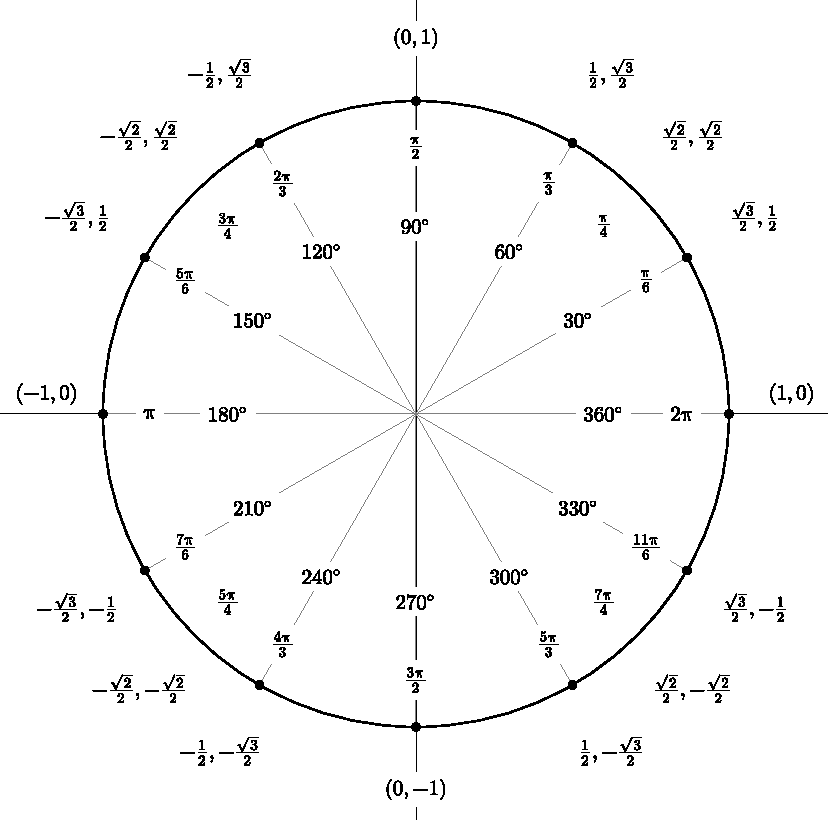
\includegraphics[width=\linewidth]{include_degrees_circle.pdf}
  
\end{center}

\section{Tabellen}
\subsection{Ableitungen}
\begin{center}
  % the c>{\centering\arraybackslash}X is a workaround to have a column fill up all space and still be centered
  \begin{tabularx}{\linewidth}{c>{\centering\arraybackslash}Xc}
    \toprule
    $\mathbf{F(x)}$ & $\mathbf{f(x)}$ & $\mathbf{f'(x)}$ \\
    \midrule
    $\frac{x^{-a+1}}{-a+1}$ & $\frac{1}{x^a}$ & $\frac{a}{x^{a+1}}$ \\
    $\frac{x^{a+1}}{a+1}$ & $x^a \ (a \ne 1)$ & $a \cdot x^{a-1}$ \\
    $\frac{1}{k \ln(a)}a^{kx}$ & $a^{kx}$ & $ka^{kx} \ln(a)$ \\
    $\ln |x|$ & $\frac{1}{x}$ & $-\frac{1}{x^2}$ \\
    $\frac{2}{3}x^{3/2}$ & $\sqrt{x}$ & $\frac{1}{2\sqrt{x}}$\\
    $-\cos(x)$ & $\sin(x)$ & $\cos(x)$ \\
    $\sin(x)$ & $\cos(x)$ & $-\sin(x)$ \\
    $\frac{1}{2}(x-\frac{1}{2}\sin(2x))$ & $\sin^2(x)$ & $2 \sin(x)\cos(x)$ \\
    $\frac{1}{2}(x + \frac{1}{2}\sin(2x))$ & $\cos^2(x)$ & $-2\sin(x)\cos(x)$ \\
    \multirow{2}*{$-\ln|\cos(x)|$} & \multirow{2}*{$\tan(x)$} & $\frac{1}{\cos^2(x)}$  \\
    & & $1 + \tan^2(x)$ \\
    $\cosh(x)$ & $\sinh(x)$ & $\cosh(x)$ \\
    $\log(\cosh(x))$ & $\tanh(x)$ & $\frac{1}{\cosh^2(x)}$ \\
    $\ln | \sin(x)|$ & $\cot(x)$ & $-\frac{1}{\sin^2(x)}$ \\
    $\frac{1}{c} \cdot e^{cx}$ & $e^{cx}$ & $c \cdot e^{cx}$ \\
    $x(\ln |x| - 1)$ & $\ln |x|$ & $\frac{1}{x}$ \\
    $\frac{1}{2}(\ln(x))^2$ & $\frac{\ln(x)}{x}$ & $\frac{1 - \ln(x)}{x^2}$ \\
    $\frac{x}{\ln(a)} (\ln|x| -1)$ & $\log_a |x|$ & $\frac{1}{\ln(a)x}$ \\
    \bottomrule
  \end{tabularx}
\end{center}
\subsection{Weitere Ableitungen}
\begin{center}
  \begin{tabularx}{\linewidth}{>{\centering\arraybackslash}X>{\centering\arraybackslash}X}
    \toprule
    $\mathbf{F(x)}$ & $\mathbf{f(x)}$ \\
    \midrule
    $\arcsin(x)$ & $\frac{1}{\sqrt{1 - x^2}}$ \\
    $\arccos(x)$ & $\frac{-1}{\sqrt{1 - x^2}}$ \\
    $\arctan(x)$ & $\frac{1}{1 + x^2}$ \\ 
    $x^x \ (x > 0)$ & $x^x \cdot (1 + \ln x)$ \\
    \bottomrule
  \end{tabularx}
\end{center}
\subsection{Integrale}
\begin{center}
  \begin{tabularx}{\linewidth}{>{\centering\arraybackslash}X>{\centering\arraybackslash}X}
    \toprule
    $\mathbf{f(x)}$ & $\mathbf{F(x)}$ \\
    \midrule
    $\int f'(x) f(x) \dx$ & $\frac{1}{2}(f(x))^2$ \\
    $\int \frac{f'(x)}{f(x)} \dx$ & $\ln|f(x)|$ \\
    $\int_{-\infty}^\infty e^{-x^2} \dx$ & $\sqrt{\pi}$ \\
    $\int (ax+b)^n \dx$ & $\frac{1}{a(n+1)}(ax+b)^{n+1}$ \\
    $\int x(ax+b)^n \dx$ & $\frac{(ax+b)^{n+2}}{(n+2)a^2} - \frac{b(ax+b)^{n+1}}{(n+1)a^2}$ \\
    $\int (ax^p+b)^n x^{p-1} \dx$ & $\frac{(ax^p+b)^{n+1}}{ap(n+1)}$ \\
    $\int (ax^p + b)^{-1} x^{p-1} \dx$ & $\frac{1}{ap} \ln |ax^p + b|$ \\
    $\int \frac{ax+b}{cx+d} \dx$ & $\frac{ax}{c} - \frac{ad-bc}{c^2} \ln |cx +d|$ \\
    $\int \frac{1}{x^2+a^2} \dx$ & $\frac{1}{a} \arctan \frac{x}{a}$ \\
    $\int \frac{1}{x^2 - a^2} \dx$ & $\frac{1}{2a} \ln\left| \frac{x-a}{x+a} \right|$ \\
    $\int \sqrt{a^2+x^2} \dx $ & $\frac{x}{2}f(x) + \frac{a^2}{2}\ln(x+f(x))$ \\
    \bottomrule
  \end{tabularx}
\end{center}

% end of larger array spacing
\endgroup
\section{Quellen}
Ein Grossteil des Cheatsheets wurde stark vom Cheatsheet von \href{https://github.com/dannycamenisch}{Danny Camenisch} inspiriert. Ausserdem stammen Teile der Tabellen aus dem Buch ``Formeln, Tabellen und Konzepte''. Die Definitionen sind meistens dem Skript ``Analysis 1'' von Marc Burger und dem Skript ``Analysis 2'' von E. Kowalski entnommen.
\end{document}